\documentclass[12pt,runningheads]{llncs}
\usepackage{graphicx}
\usepackage[
    left=3cm,
    right=3cm,
    top=4cm,
    bottom=4cm
]{geometry}
\usepackage{etoolbox}
\usepackage{array}
\usepackage{fontspec}

\setmainfont{FreeSerif}

\apptocmd{\thebibliography}{\setlength{\itemsep}{12pt}}{}{}

\begin{document}

% --------------------------------------------------------------------------- %
\title{CMP3753 Literature Review and Progress Update}

\author{Luke Roberts}

\institute{University of Lincoln \\
    \email{\textrm{25722923@students.lincoln.ac.uk}}
}

\maketitle

\begin{figure}[h]
    
\includegraphics[scale=0.7]{UOL_Logo.jpg}
    \centering
\end{figure}

\newpage
% --------------------------------------------------------------------------- %

\section{Literature Review}

\noindent As specified in the project proposal (L. Roberts 2023) the project aim
is to compare the ability of different convolutional neural network (CNN)
architectures to classify the morphology of galaxies. Images and
classifications from the NASA/IPAC Extragalactic Database (NED) will be
used to train and test the performance of each model. This literature
review serves to inform the reader about the background of CNNs and
personal considerations in choosing the models that will be tested in
this project.

\subsection{Early Convolutional Neural Networks}
CNNs are a specific type of machine learning model that aims to
classify images as well as other kinds of unstructured data. While much
more commonplace in studies today, CNNs have existed since the late
1980s. (Y. LeCun et. al, 1989) developed a CNN called LeNet
which successfully categorised handwritten digits with a 3.4\% error
rate. The study, undertaken in AT\&T Bell Labs, pioneered the
utilisation of `convolutional feature maps' for feature abstraction in
higher hidden network layers, which are still a core component of CNN
architectures. Since CNN architectures derive from artificial neural
networks, training LeNet is undertaken through forward propagation
and back propagation.

LeCun and his colleagues continued their research throughout the next
decade, incrementally improving on the design of LeNet. In the paper
(Yann LeCun et. al, 1998), LeNet-5 architecture improved upon the
original model by adding more alternating convolution and subsampling
layers, and traditional neural network layers using full connections
before the output layer. LeNet-5 also used a minimisation procedure
for backpropagation called stochastic gradient descent, which minimises
parameter vectors around the local minimum at greater speeds than more
traditional gradient descent algorithms, improving model training speed
greatly. While relatively simple, LeNet-5 has been used in many
practical applications across many fields of study. Indeed, a 2022
conference paper (P. S. Radhamani et. al 2022) showed that
LeNet-5 was capable of categorising galaxy morphology with 96\%
accuracy for two classes. However, the statistic found in the conclusion
is misleading because the paper intended to categorise nine different
classifications, and did so with varying degrees of success.
Nevertheless, because of its implementation simplicity and historic
relevance the LeNet-5 architecture will be used as a baseline CNN in
the project for comparison to more recently designed CNN architectures.

\newpage
\subsection{Developments in Convoluted Neural Networks}
Although LeNet-5 was a breakthrough for CNN architecture, neural
networks had yet to be widely used in research and commercial settings.
This was largely due to the limitations the hardware could provide at
the time -- only high end hardware could run the number of complex
matrix multiplication operations needed for LeNet-5, limiting the
scope and number of projects using the architecture. As hardware
continued to improve through the 2000s and early 2010s, deep CNNs became
more accessible, meaning scope of CNN-based projects became larger and
more widespread. One pioneering architecture was AlexNet by (A.
Krizhevsky et. al 2017), originally trained on the ImageNet dataset
for the ImageNet Large Scale Visual Recognition Challenge 2012.
Compared to earlier models such as LeNet-5, AlexNet was much
more deep, containing five convolution layers and three full layers.
This meant that the neural network had the potential to learn patterns
of greater abstraction about the input dataset. However, because of the
increase in model depth, new techniques were also employed to mitigate
the impact of a CNN training issue called the vanishing gradient
problem. (S. Basodi et. al 2020) describe the vanishing gradient problem
as when ... during backpropagation, network weights are updated
proportional to the gradient value (...) after each training iteration
(epoch). \ldots, sometimes the gradient value is too small and gets
gradually diminished during backpropagation to the initial layers.' In
more understandable terms, as backpropagation trains layers that are
closer to the input layer less. To facilitate continued training of
AlexNet, a ReLU activation function was used instead of a sigmoid
function. AlexNet continues to be used as an image categorisation
model because of its lower computational needs and its high
performance.

After the success of AlexNet in 2012, there was a renewed interest
in deep learning models for use in computer vision and other domains.
New breakthroughs in CNN architectures became much more frequent and the
depth of new models continued to increase. A problem that was addressed
by S. (Basodi et. al 2020) was that the gap of error between networks
with 18 and 34 layers converged after a certain number of iterations
known as the degradation problem. They discovered that by using residual
connections between layers, the 34 layer model performed better
throughout all training iterations. The model they developed became
known as ResNet, which has been used in many practical applications
for image categorisation. Both ResNet and AlexNet are modern CNN
architectures which will be tested as part of the project; comparing the
abilities of a modern but simpler model to a deeper residual network
architecture.

A similar study involving morphology categorisation of galaxies from
Galaxy Zoo 2 by (J. Dai, J. Tong. 2018) showed that implemented
ResNet-50 and AlexNet models could achieve \textgreater90\%
accuracy. That being said, the best performance was achieved by their
custom designed model. ResNet and AlexNet have
been selected for this project alongside the LeNet-5 model to test
how different architectures affect model performance.

\newpage
\section{Progress Report}
As planned in the objectives of the project proposal (L. Roberts 2023)
the first step of the project was to collect a dataset of images and
classifications using the python astronomy database querying tool AstroQuery.
AstroQuery allows the user to interface with many online astronomy databases
including the European Space Agency Hubble Space Telescope (ESA HST)
Archive and the NASA/IPAC Extragalactic Database (NED). The NED archive
was chosen because it compiled different records of galaxies from separate
observatories, having \~2,500,000 images (NED Current Holdings n.d.) as 
of its most recent release.

My initial AstroQuery experimentation was done on a Jupyter Notebook 
(Jupyter 2019) because of its ability to interface with scientific computing
libraries. Firstly image downloading was tested using the Ned.get\_images function. 
Using the python scientific diagram library MatPlotLib (Matplotlib 2012),
the images downloaded from the archive could be displayed. The specific
file format that the NED database contains are Flexible Image Transport System 
(FITS) images.

\begin{figure}[h]
    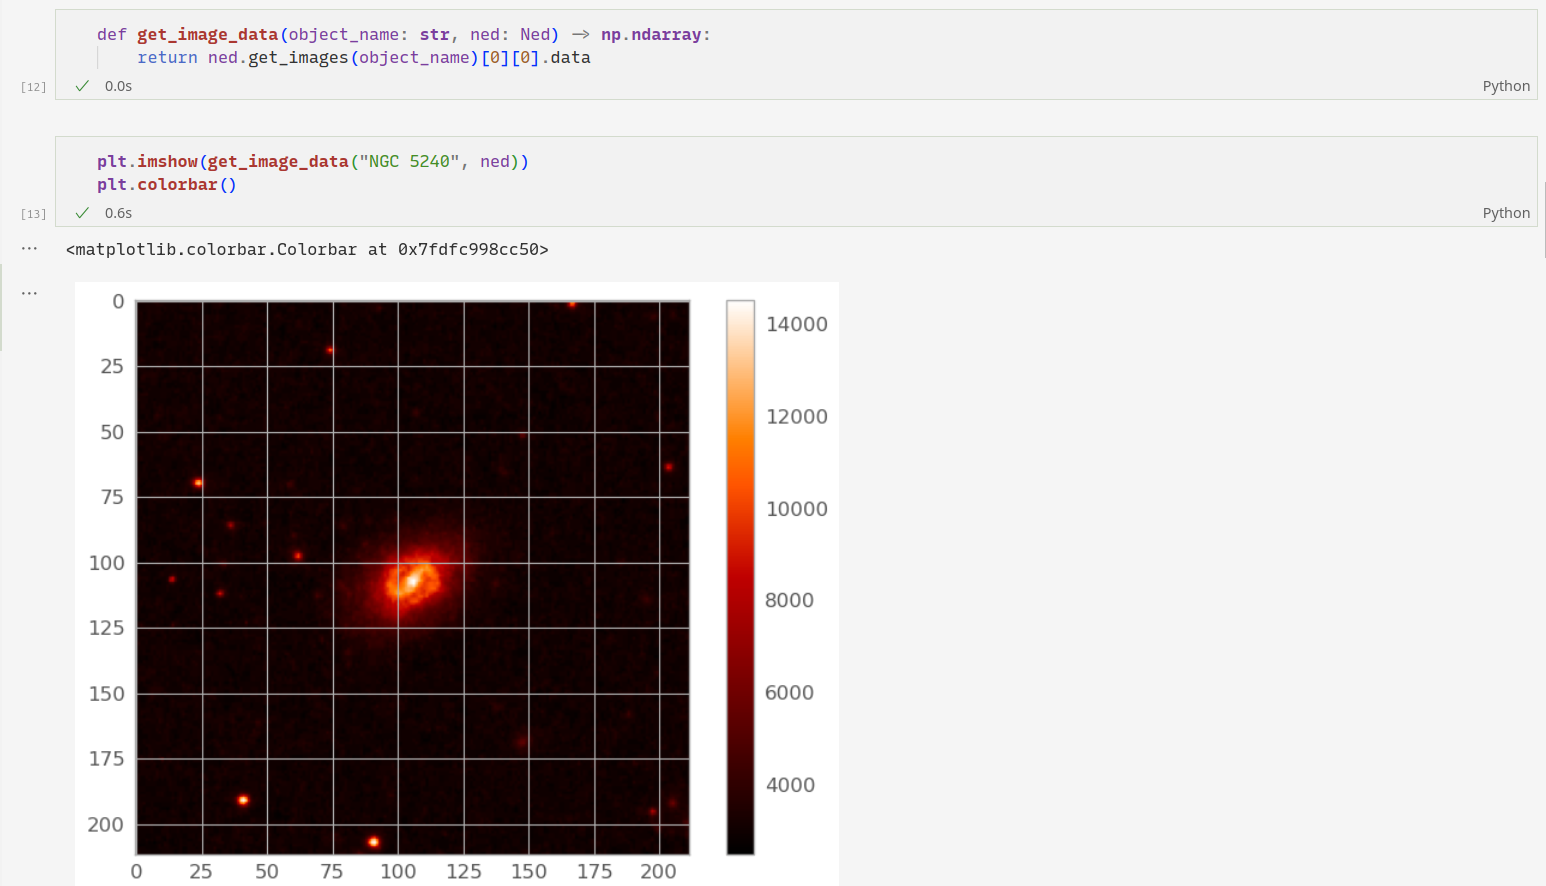
\includegraphics[scale=0.3]{Screenshot_2024-01-31_21-26-47.png}
    \centering
    \caption{Output image from NED using astroquery}\label{tab1}
\end{figure}

\noindent Once image acquisition was tested, the next step was to query for a table of galaxy
names and each galaxy's associated classification using Ned.get\_table. Unfortunately
the NED API implemented for AstroQuery did not return a column for galaxy classification 
when tested. 

\begin{figure}[h]
    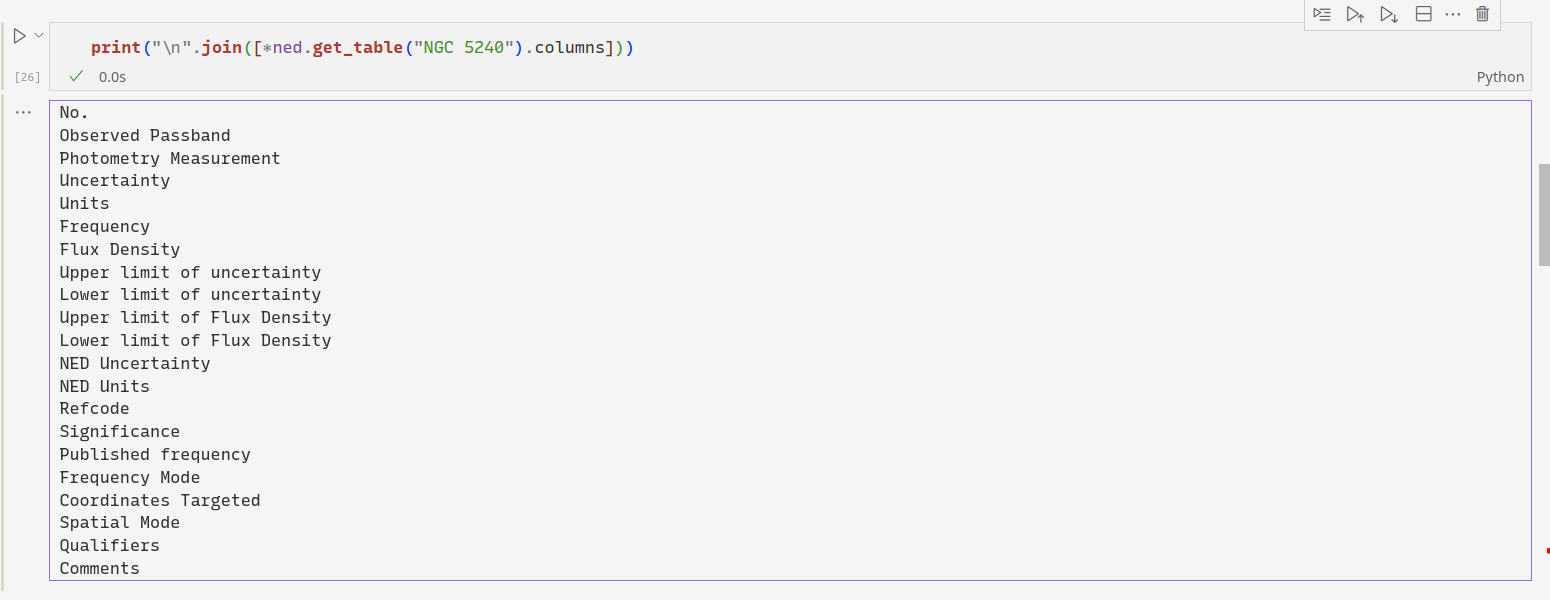
\includegraphics[scale=0.3]{Screenshot_2024-01-31_23-37-59.png}
    \centering
    \caption{Output showing no classification column}\label{tab1}
\end{figure}

\noindent The API reference was consulted to determine a way to configure the NED database search,
however, nothing that was tried gathered the classifications. A risk that was discussed
in my project proposal was that ‘an external database [was] unavailable’ which is similar
to the issue that was currently being faced; not having part of the database available.
Since it was unlikely that the API would be updated, the contingency was to use a different
database meaning that a table containing both object names and classifications had to be
collected from a different source. It was preferable to keep using NED as there would
be a set of both names and images so more research was directed to find a source using
NED. Luckily, there was an old online search tool that allowed specific classifications
and object names to be searched (NED Search by Classifications) however, it only outputted
a HTML table on many separate pages. The issue was resolved by writing a web scraping
script to get-request every page given certain search criteria. The webpage had to be
inspected in the browser so that each web page input that was needed was included as an 
option. The text from the requested page was then parsed into a dataframe, joined to other
queries and exported as ‘NED\_list.csv’. To maximise efficiency, a thread pool executor was
used to parallelise the process of searching for pages.

\begin{figure}[h]
    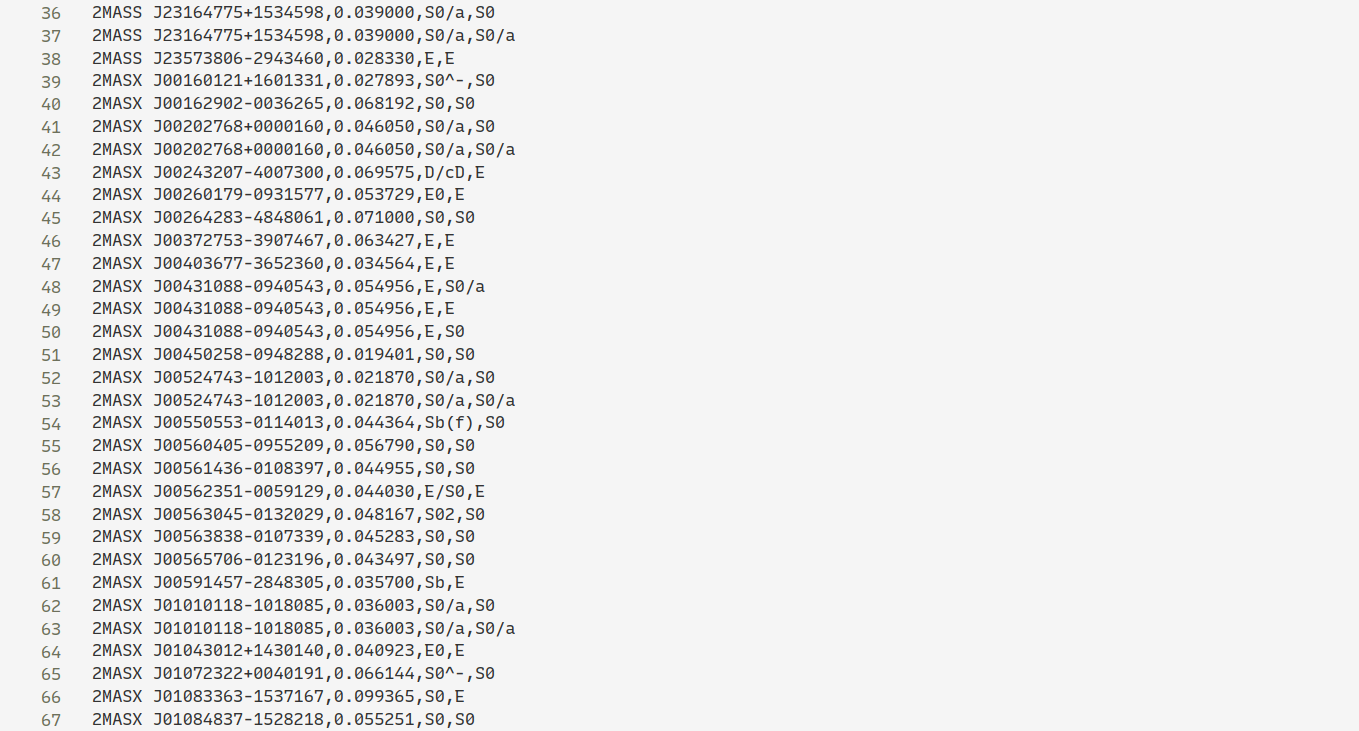
\includegraphics[scale=0.3]{Screenshot_2024-02-01_03-39-05.png}
    \centering
    \caption{Output table showing object and classification}\label{tab1}
\end{figure}

\newpage

\noindent After creating the table of galaxies and morphologies a tool was then developed to gather
images from the NED archive. This tool used Ned.get\_image\_list to find if there were valid
files available and took the name of the highest quality image file (always indexed at one
from testing). FileContainer.get\_fits was used to download the files individually and then
HDUList.writeto wrote the data to a file. I then wrote another script that displayed each
image for illustrative purposes.

\begin{figure}[h]
    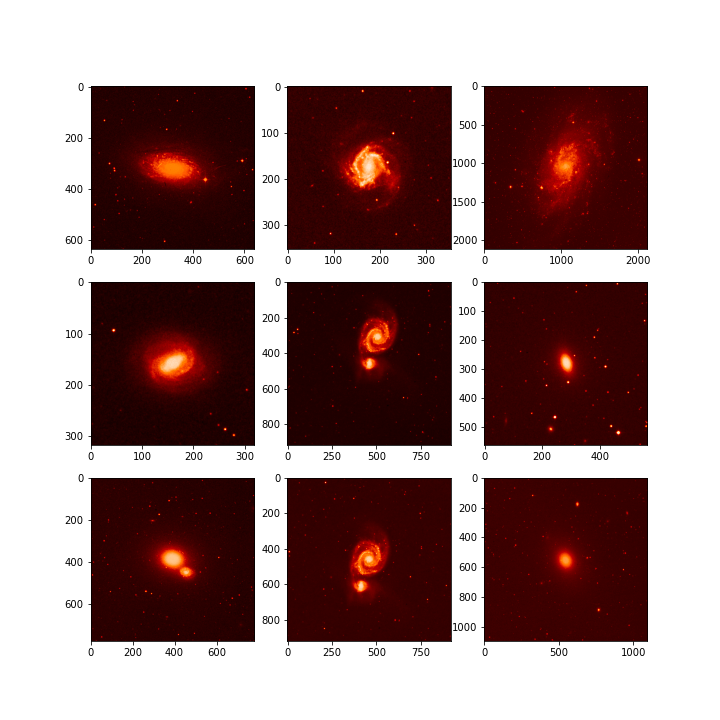
\includegraphics[scale=0.4]{Figure_1.png}
    \centering
    \caption{Images downloaded from NED archives}\label{tab1}
\end{figure}

\noindent The next project steps will be preprocessing images of the dataset and building the machine
learning models for testing. In the project objectives, the next stage after dataset gathering
was to analyse the images and dataset to determine how best to perform preprocessing. 
One issue with many of the images is that most of the image is empty space, which a machine 
learning model will find redundant when trying to categorise the image. Similar to the 
preprocessing performed in figure 6 of (J. Dai, J. Tong. 2018), each image will be cropped 
to a specific scale. Another issue present in the image dataset is that images range greatly 
in quality. To be able to input each image for training and testing, each image will be 
downscaled to a specific size and images with quality below a certain threshold will be removed, 
as they are unlikely to be useful in training. In the database, there are many galaxy objects 
that appear in two or more astronomical catalogues (MESSIER, NGC, ESO, etc.), so to prevent 
any biases that could occur only one catalogue will be used to train the models that will be 
implemented.

\newpage
\noindent Overall progress has been slower due to other university work, commitments and the setbacks 
discussed in this section. However, more focus can now be drawn to CNN model creation and 
preprocessing for the project, now that data gathering is completed. All of my current code
and testing notebooks can be found on the github repository (Luke-A-C-Roberts 2024).


% --------------------------------------------------------------------------- %

\begin{thebibliography}{20}

\bibitem{}
L. Roberts (2023) “CMP3753M Project Proposal”. University of Lincoln, School of Computer Science. Unpublished essay.

\bibitem{}
Y. Lecun, B. Boser, J. Denker, D. Henderson, R. Howard, W. Hubbard, and L. Jackel (1989) “Backpropagation applied to handwritten zip code recognition”. IEEE, Available at: https://ieeexplore.ieee.org/document/6795724

\bibitem{}
Y. Lecun, L. Bottou, Y. Bengio, P. Haffner (1998) “Gradient-based learning applied to document recognition”. IEEE. Available at: https://ieeexplore.ieee.org/document/726791

\bibitem{}
P. Radhamani, M. Sharif and W. Elmedany (2022) “An Effective Galaxy Classification Using Fractal Analysis and Neural Network” International Conference on Innovation and Intelligence for Informatics, Computing, and Technologies (3ICT). Available at: https://ieeexplore.ieee.org/document/9990776

\bibitem{}
A. Krizhevsky, I. Sutskever, G. Hinton (2017) “ImageNet Classification with Deep
Convolutional Neural Networks”. ACM Digital Library. Available at: https://dl.acm.org/doi/10.1145/3065386\#sec-ref

\bibitem{}
S. Basodi, C. Ji, H. Zhang and Y. Pan, (2020) “Gradient amplification: An efficient way to train deep neural networks,” in Big Data Mining and Analytics. Available at: https://ieeexplore.ieee.org/document/9142152

\bibitem{}
K. He, X. Zhang, S. Ren and J. Sun, (2016) “Deep Residual Learning for Image Recognition”, IEEE Conference on Computer Vision and Pattern Recognition (CVPR). Available at: https://ieeexplore.ieee.org/document/7780459

\bibitem{}
J. Dai, J. Tong. (2018) “Galaxy Morphology Classification with Deep Convolutional Neural Networks”, Tables 6-7, arXiv (preprint). Available at: https://arxiv.org/pdf/1807.10406.pdf

\bibitem{}
NASA/IPAC Extragalactic Database. (n.d.) “Database holdings for release 33.3.1”. [online] Available at: http://ned.ipac.caltech.edu/CurrentHoldings

\bibitem{}
Jupyter (2019). Project Jupyter. [online] Jupyter.org. Available at: https://jupyter.org/

\bibitem{}
NASA/IPAC Extragalactic Database. (n.d.) “Search by Objects” https://ned.ipac.caltech.edu/uri/NED::Classifications/\#M

\bibitem{}
Matplotlib (2012). Matplotlib: Python plotting — Matplotlib 3.1.1 documentation. [online] Matplotlib.org. Available at: https://matplotlib.org/

\bibitem{}
Luke-A-C-Roberts (2024). Luke-A-C-Roberts/Project. [online] GitHub. Available at: https://github.com/Luke-A-C-Roberts/Project [Accessed 1 Feb. 2024].

\end{thebibliography}

\end{document}

% --------------------------------------------------------------------------- %
